\documentclass[../main.tex]{subfiles}
\begin{document}

\chapter{Preventing unauthorized access}

\section{Introduction}
\subsection{Access control in web applications}
\begin{itemize}
\item Authentication is only the first step
\item Authentication in web applications is one of these topics with a long history. Everybody has their idea of how to do it, and most of these ideas are antiquated.
\item Also storing credentials is harder then you would think.
\item Using multi-factor authentication also provides several benefits.
\item Many applications keep track of the user's authenticated state in a session object. Sadly most of them fail to get the details of secure session management right.
\item On the one hand, the application needs to enforce proper permissions on access to data or operations. But on the other hand, the application also needs to ensure that actions carried out in the user's name are intentional.
\end{itemize}

\subsection{Introducing state into your application}
\begin{itemize}
\item HTTP is a stateless protocol $\rightarrow$ authentication and authorization are challenging.
\item \textbf{HTTP Basic Authentication}
\begin{enumerate}
\item Server tells browers that a resource is off limits.
\item Browser will prompt the user to authenticate.
\item With the user's credentials, the browser again tries to fetch the resource. The credentials are present in the Authorization header.
\item The server can now verify the credentials and decide if the user can access the resource. If the answer is affirmative, the response has \textbf{status code 200} and contains the resource. Otherwise, the server can send an error message with \textbf{status code 403}.
\end{enumerate}
\item Note that the Authorization header does not contain the cleartext credentials. The browser has \textbf{base64-encoded} them to ensure they can be safely used in an HTTP message $\rightarrow$ can easily be undone, not for security reasons. Because it is sent as part of the request, and passwords can contain any kind of characters. Some of these characters could confuse the server parsing the headers, resulting in vulnerabilities.
\item Drawbacks:
\begin{enumerate}
\item it provides only the identity of the user $\rightarrow$ no support to track additional properties
\item The username and password are present in every request $\rightarrow$ All an eavesdropper needs to impersonate the user is to capture one request.
\item Once entered by the user, the browser keeps using the credentials for that website. The only effective way for the user to log out is to close the browser.
\item The browser handles authentication in a popup window. As a consequence, the authentication form cannot be integrated into the application's UI.
\end{enumerate}
\item Today, most applications use a custom authentication form, in combination with session management.
\item Session management ensures the propagation of authentication information.
\item Unfortunately, this complex configuration is prone to mistakes and misconfigurations. Many applications suffer from broken authentication and session management. These issues are quite severe, as they result in unauthorized access to the application. The OWASP top 10 even ranks them in second place.
\end{itemize}

\section{Secure authentication}
\subsection{The truth about passwords}
\begin{itemize}
\item More and more voices are proclaiming passwords as insecure, inefficient or even outright evil. They advocate the use of alternative authentication mechanisms, such as hardware tokens or mobile applications. $\rightarrow$ but complicated and disruptive.
\item Almost every application today still uses passwords.
\item One of the weakest security properties of a password is that it is usable by anybody that knows it.
\item Various kinds of attacks.
\begin{itemize}
\item Guess the password, using a variety of techniques (using personal information, dictionary attacks, lists of commonly used passwords,...)
\item \textbf{phishing attack}: tricks the user into visiting a malicious website. This website looks exactly like an innocent one. When the user authenticates to the malicious site, the attacker steals the user’s credentials.
\item Hacking the application and stealing the database $\rightarrow$ many applications store passwords in an insecure way.
\end{itemize}
\item These attacks are amplified by the fact that many people reuse passwords across accounts. Everyone has dozens of accounts with a password, and remembering a unique password for each account is next to impossible. As a result, obtaining a single password gives the attacker access to many accounts of the same user. The increase in data breaches has resulted in massive online dumps of credentials.
\item The problem is so bad that there is even a website keeping track of all the accounts in the data dumps. The site is \textbf{Have I Been Pwnd}, and it allows you to see if your email address occurs anywhere in the set of data dumps.
\item The best way to improve the security of passwords is by using a \textbf{password manager}. A password manager is an application that securely stores credentials for various accounts. The biggest benefit is that the user no longer needs to remember them. As a result, password managers enable the use of a unique and complex password for every account.
\item Eliminates security problems.
\begin{enumerate}
\item Guessing attacks become irrelevant, since passwords can now be long and random.
\item There is no longer a need reuse passwords across accounts.
\item Increase the resilience against phishing attacks. Many password managers offer autocomplete features in the browser. But in a phishing attack, the URL points to a malicious site, so the password manager will not find any associated accounts.
\end{enumerate}
\item If you don't want to use a password manager, you can take some countermeasures as well (e.g. divide accounts into trust levels, and use a different password for each of these levels).
\end{itemize}

\subsection{Insecure password storage}
\begin{itemize}
\item One of these weak behaviour patterns is reusing passwords across many applications.
\item It is best to adhere to a defense-in-depth strategy to minimize the impact of a data breach $\rightarrow$ Store your passwords securely!
\begin{enumerate}
\item \textbf{Plain text}: problematic in light of a data breach, attacker has full access. 
\item \textbf{Hashed (MD5,SHA1...)}: two users pick same password $\rightarrow$ same hash + \textbf{rainbow tables}: tables of precomputed hashes of commonly used passwords $\rightarrow$ retrieving passwords from the stolen data becomes trivial.
\item \textbf{Hashed with salt}: long, random string per user, that is appended to the password before it is hashed. The application stores the salt in the database, alongside the hash of the password. During authentication, the application recomputes the hash with the plaintext password and the salt. If the hash matches the stored hash, the user has provided the original password $\rightarrow$ precomputation attacks are infeasible.\\
\emph{But:} It is weaker than you might expect. Hashing algorithms are designed to be fast $\rightarrow$ brute force attack to try out each of the passwords with all the salts. This approach is not infeasible using modern-day GPU-based password cracking software.
\end{enumerate}
\end{itemize}

\subsection{Secure password storage}
\begin{itemize}
\item To prevent brute force attacks, you should use a dedicated password hashing function. These are cryptographic functions that perform a certain amount of iterations to calculate the output. As a result, they are expensive to execute, and withstand brute force attacks by design. In practice, all recommended password hashing functions also use a salt to ensure that even if two users pick the same password, the hash will be different.
\item Popular dedicated password hashing functions: \textbf{bcrypt, argon2, PBKDF2, scrypt...}
\item The output of the bcrypt function contains several parts: 
\begin{enumerate}
\item The first part indicates which algorithm has generated the hash.
\item The second part specifies a \textbf{cost parameter} (makes the function more expensive to execute).
\item The third part contains a salt and the resulting hash.
\end{enumerate} 
\item For a cost factor of 5, a very powerful machine (8 Nvidia GTX GPUs) can only calculate 100 000 hashes per second.
\begin{figure}[h!]
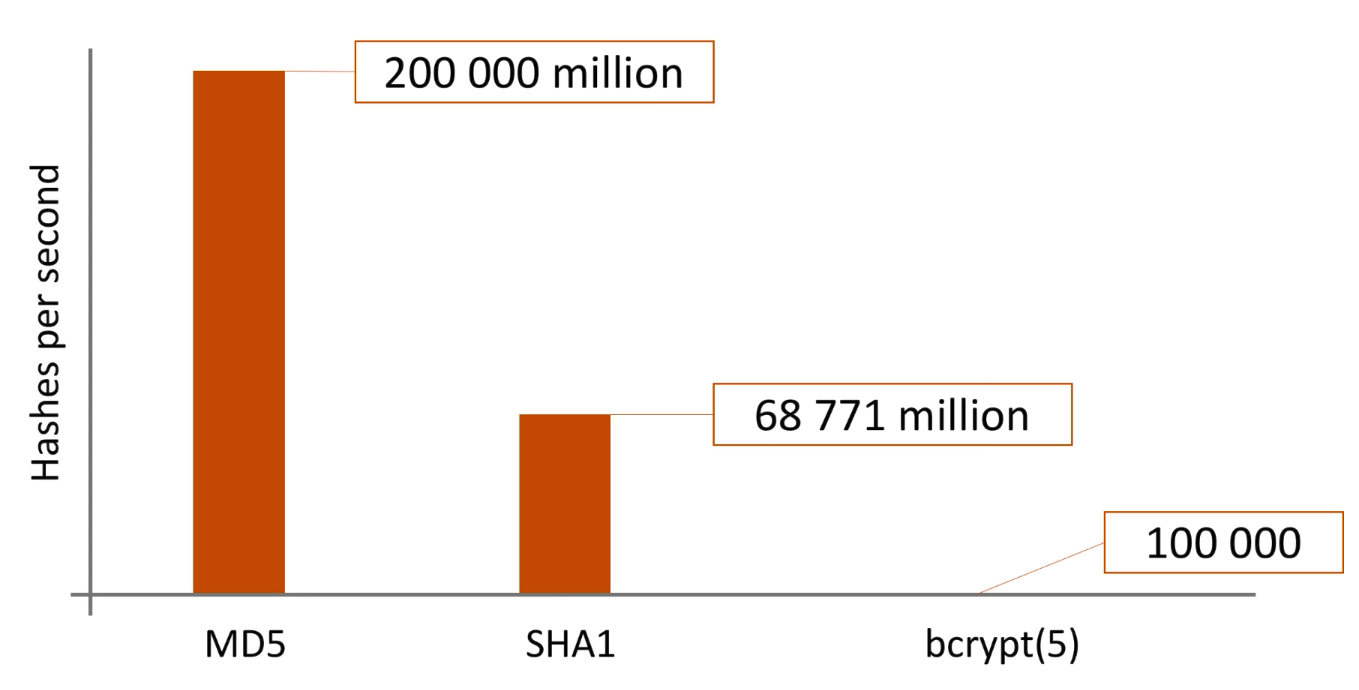
\includegraphics[width=\textwidth]{../images/bcrypt}
\caption{Comparison between MD5, SHA1 and bcrypt (cost factor 5) on system with 8 Nvidia GTX GPUs}
\end{figure}
\item Note that the cost factor is exponential and that the current recommendations list 12 as a minimum.
\item There are a few strategies you can follow to upgrade the storage mechanism.
\begin{enumerate}
\item \textbf{Gradual upgrade path}: When the user has provided a valid password, the application checks how the password is stored in the database. When the stored hash is calculated with a legacy algorithm, it needs to be updated. The application uses the password to calculate a bcrypt hash, and stores the new hash in the database. Running this gradual upgrade strategy for a couple of months will replace the stored hashes for all your active users. At a certain point in time, it makes sense to reset the passwords on all accounts that have not yet been upgraded. If users want to resume their account, they can use the account recovery process.
\item \textbf{Drastic update}: Imagine that you have a database full of unsalted MD5 hashes. If you want to upgrade your application to bcrypt, you can use the MD5 hashes as input for the bcrypt function. The database now contains bcrypt hashes of MD5 hashes of the plaintext password. For the authentication procedure you first have to check the validity of the provided password by double hashing it. Next, you use the plaintext password to calculate a single bcrypt hash and replace the double hash with the newly generated one.
\end{enumerate}
\end{itemize}

\subsection{Preventing enumeration attacks}
\begin{itemize}
\item In a \textbf{brute force attack}, the attacker tries to guess the password of a valid user of the application $\rightarrow$ can be very effective!
\item With an \textbf{enumeration attack}, the attacker can determine if a username exists in the application. If the application leaks such information, it can be abused to compile a list of valid usernames. That list, in turn, enables the attacker to optimize his brute force attack.
\item Where does an application leak usernames?
\begin{enumerate}
\item \textbf{Authentication forms}: Don't choose an error message that reveals whether a username exists or not.\\
\emph{Fix:} Avoid leaking information about the existence of an account.
\item \textbf{Account recovery form}: More often than not, it immediately notifies the user when the email address is not found.\\
\emph{Fix:} The first step is to refrain from giving the user immediate feedback about the existence of an email address. Instead, you look up if an email address exists. If it exists, you send the recovery email, like before. If it does not exist, you can send a message that informs the user about the potential account recovery. You can point out that the user may have used a different email address to sign up. Alternatively, you can suggest that the user can always register a new account if desired.
\item \textbf{registration form}: When choosing a username or email address, the application discloses if it already exists.\\
\emph{Fix:} The simple case is when the application uses email addresses as a unique identifier. In this case, you can implement a similar mechanism as for recovery. If the email address is not yet known to the application, you create a new account and send an email to the user. If the email address matches an existing account, you send an email to remind the user of this account. You should also include instructions on how to recover the password. Things become a lot more complicated if the application uses arbitrary identifiers, such as usernames. The application will have to enforce uniqueness across the entire userbase. However, these identifiers are chosen by the user. One way to limit this risk is to require registration with an email address first. Only then allow the selection of a username. This allows you to impose a limit on the number of attempts to pick a username. As a result, the attacker can only learn a tiny amount of information during an attack.
\end{enumerate}
\item There are two common strategies to prevent brute force attacks.
\begin{enumerate}
\item Lock a user account after a certain number of authentication attempts $\rightarrow$ How will you distinguish a forgetful user from an attacker? Will you need to manually intervene to unlock an account? What happens if an attacker locks all accounts in your application?
\item Slow down authentication attempts after a couple of failures $\rightarrow$ increasing the slowdown makes a brute force attack infeasible.
\end{enumerate}
\end{itemize}

\subsection{Beyond password-based authentication}
\begin{itemize}
\item Passwords are a weak form of authentication $\rightarrow$ other means of authentication exist as well (possession of a physical device, biometrics, behavior and context...).
\item \textbf{Multi-factor authentication}: Using an alternative authentication method in combination with a knowledge-based authentication.
\item E.g. The combination of a username and password with an SMS-based verification code.
\begin{itemize}
\item The user links a mobile phone number with his account. When the user logs in, the application sends a random verification code to the phone number. The user enters this code into the second login form, and the application compares if the codes match.
\item At first sight, an SMS-based verification code seems very secure.
\item But because this scheme makes a lot of assumptions, it suffers from a variety of weaknesses.
\begin{enumerate}
\item If the user stores his password on his smartphone, the attacker only needs to access the phone.
\item An attacker setting up a phishing site can still trick the user.
\item If the attacker can take control of the phone number, he can receive the verification code (tricking phone company or abusing the underlying cellular protocols).
\end{enumerate}
\item No longer recommended to use a mobile phone number as an authentication factor.
\end{itemize}
\item E.g. The use of a U2F security key.
\begin{itemize}
\item \textbf{U2F} stands for \textbf{Universal Second Factor}, and is an open standard for device-based authentication on the web (e.g. \textbf{Yubikey}).
\item Supported by numerous major application providers, including Google and Facebook.
\item To use a U2F device, the user first registers it with his account. From then on, the second step in the authentication process is inserting the U2F key and touching the device. The device will use an embedded secret to sign a challenge, proving to the application that it is the same device as registered before. Multi-factor authentication with U2F devices is a secure scenario. The successful signing of a challenge indicates the possession of a previously registered key. The touching of the U2F device indicates a physical presence of the user. This step makes it much harder for malware to trick the device into signing a challenge. Additionally, the origin of the context where the authentication happens is part of the signature. 
\item Not susceptible to phishing.
\end{itemize}
\item But companies such as Google and Facebook have already implemented all of this, and probably better than you ever can. Why not use this? $\rightarrow$ outsourcing of authentication to third parties (\textbf{social login}).
\item Under the hood, delegating authentication often depends on the use of \textbf{OAuth 2.0} or \textbf{OpenID Connect}.
\begin{enumerate}
\item When the user opts for a social login, the application redirects the user to the third-party authentication provider.
\item If the user is not logged in, the provider will trigger its own authentication procedure.
\item Once authenticated, the provider verifies whether the user allows the use of social login for our application. When allowed, the authentication provider redirects the flow back to our application, and passes a security token as part of the URL.
\item With this token, our application can request information about the user from the provider. This information allows our application to identify the user.
\end{enumerate}
\item Implementing multi-factor authentication a considered a best practice today, but it requires a significant amount of effort. A good alternative is delegating authentication to third-party providers.
\item Implementing this in practice poses many challenges, and lots of insecure implementations exist!
\end{itemize}

\section{Challenges to session management}
\subsection{Server-side session management}
\begin{itemize}
\item Server-side session management is the de facto standard.
\item This traditional way of keeping state in a web application depends on storing information in a session object on the server. Each session object has a unique identifier (\textbf{session identifier}, or \textbf{SID}), which is shared with the client. When the browser includes this identifier in every request, the server can tie multiple requests together in a session.
\item Several strategies for including the session identifier in every request.
\item The most common strategy is to store the session identifier in a cookie. The browser automatically attaches the cookie on every request. The use of cookies results in a robust session management mechanism.
\item An alternative strategy is to include the identifier in every URL in every page. While this approach works in practice, it is less recommended. Reasons are a higher level of complexity, and a higher risk of leaking the session identifier to third parties.
\item \emph{Traditional cookie-based session management mechanism:}
\begin{enumerate}
\item When the user first opens the application, there is no session.
\item So when the server receives the first request, it generates a new session object (with an assigned session identifier).
\item The server sends this session identifier back to the browser. From now on, every request from the browser to the server will include this identifier.
\item The server uses this identifier to look up the right session object and access its data.
\end{enumerate}
\item \emph{How is the session identifier stored in the cookie?}
\begin{enumerate}
\item The server sets the session cookie by sending the Set-Cookie response header. The header contains the name of the cookie, and the session identifier. There is no predefined name for a cookie containing a session identifier. Commonly used names are \textbf{SESSIONID}, \textbf{PHPSESSIONID}, \textbf{JSESSIONID} and so forth.
\item The same cookie name and value will be present in the Cookie header, which the browser attaches to outgoing requests to the same domain.
\end{enumerate}
\item The security of this session management mechanism depends on the secrecy of the session identifier. If an attacker obtains the user's session identifier, he can take control of the session.
\item Two common weaknesses that can result in the disclosure of the session identifier:
\begin{enumerate}
\item A first weakness follows from the insecure generation of a new session identifier. If a session identifier is predictable in some way, an attacker can calculate past and future identifiers. This attack is known as brute-forcing the session identifier. Applications that use a custom algorithm to generate session identifiers are often vulnerable to this attack. The proper way to generate session identifiers is to use a secure random number generator.
\item A second weakness is the insecure transmission or storage of the session identifier. Sending the session identifier in clear text over the network allows interception by an eavesdropper.
\item (Another potential attack vector is cross-site scripting.)
\end{enumerate}
\end{itemize}

\subsection{Securing session cookies}
\begin{itemize}
\item One attack vector for a session hijacking attack is eavesdropping on the network. If the application uses HTTP, it exposes the session cookie on the network $\rightarrow$ more common than you may think due to partial HTTPS deployments.
\item Just deploy the whole application over HTTPS! $\rightarrow$ the cookie with the session identifier is only sent over the secure channel. But remember, HTTP traffic can be observed and manipulated by the attacker. So when the user opens any other web page over HTTP, the attacker can alter the response. Here, he inserts an image tag to trigger an HTTP request to our application. The browser sends a request to load the image our application. This request will contain the cookies. Even though our application responds with a redirect to HTTPS, it’s already too late.\\
\emph{Fix:} The server can mark the session cookie as \textbf{secure}, which tells the browser that it should only be sent over HTTPS. In practice, the server can mark a cookie as secure by attaching the \textbf{Secure flag} to the Set-Cookie header.
\item \emph{Note:} If the application is using HTTPS in combination with a Strict Transport Security policy, this attack would also not have been possible. Even if the attacker instructs the browser to make an HTTP request, the Strict Transport Security policy will cause the request to be sent over HTTPS anyway.
\item There is a second common attack vector: stealing the cookie from JavaScript. When the attacker can control a piece of JavaScript running on a page of the application (exploiting a \textbf{Cross-Site Scripting flaw}), he can abuse this to access the cookies.\\
\emph{Fix:} The server can set another cookie flag, the \textbf{HttpOnly flag}. This flag marks a cookie as valid for network requests, but not for script-based access. So a session cookie set with the HttpOnly flag is attached to HTTP and HTTPS requests, but is not returned when accessing the \texttt{document.cookie} property. Session cookies should always be set with the HttpOnly flag enabled. In fact, it is a good idea to set the HttpOnly flag on all cookies that do not need to be accessed from JavaScript.
\end{itemize}

\subsection{Alternative session management mechanisms}
\begin{itemize}
\item Think about what would happen when an application is replicated on many servers. The first request goes to a particular server, and that server creates a session object and returns a session identifier. But what happens with the second request? That request now contains an identifier that points to a session object generated by the first server. Several strategies to tackle this problem exist.
\begin{enumerate}
\item One example is the use of \textbf{sticky sessions}, where all requests within a session go to the same server.
\item Another example is \textbf{sharing session state} between servers.
\item Many modern applications are moving from server-side session management to \textbf{client-side session management}. Session state is stored on the client instead of the server. This way, the server no longer needs to keep track of session data. This fits well within the recent move towards stateless API-based systems.
\begin{itemize}
\item When the user first opens the application, there is no session.
\item When the server receives the first request, it generates a new session object and sends this entire session object back to the browser.
\item From now on, every request from the browser to the server will include this session object.
\item The server can directly use the provided session object to access the data.
\item The information stored in the session object is crucial for making authorization decisions throughout the application.
\end{itemize}
\end{enumerate}
\item \emph{What are the security implications of client-side session management?}
\begin{enumerate}
\item The session object stored on the server is considered trusted data. With a session object stored on the client, that assumption no longer holds. The attacker can now change a session object before sending it to the application. The server should check the integrity of the session object, before using any of its data. This integrity check is often implemented by adding a server-generated signature to the session object.
\item With server-side sessions, it is straightforward to consult a list of active sessions or to revoke a specific session. With client-side sessions, this is a lot harder, or even impossible. There is no easy way to list active sessions, because these sessions are only seen when the client makes a request.
\item Revoking a specific session is also a hard problem, that is still being debated by experts in the field.
\item Many applications moved away from using cookies, and use custom headers to transport the session object. While this avoids some of the security challenges with cookies, it also complicates matters for the developer. Cookies are handled automatically by the browser, while custom headers are not. So with custom headers, the developer needs to retrieve the session object from the server, store it somewhere, and attach it to outgoing requests. The choices made to implement these operations have certain ramifications for security.
\end{enumerate}
\end{itemize}

\section{Getting authorization right}
\subsection{Authorization throughout your application}
Tips by Marten Decat to secure your application.
\begin{itemize}
\item Never trust the client.
\item Don't do any access control on the client.
\item Only use trusted data, server-side trusted data.
\item Have correct session management.
\item Have proper HTTPS transport security.
\item Many of the major frameworks these days give you primitives and support to do access control right. Don't start building it from scratch and reuse everything that is given to you.
\item Access control in general these days is often referred to as "triple A": \textbf{Authentication Authorization and Audit}.
\begin{itemize}
\item Authorization is sometimes called \textbf{a priori access control}. It's when a user makes a request to an application before actually executing the action you check by the access control rules that hold whether this user should be permitted to do this action, and if not you just don't do it.
\item Audit is called \textbf{a posteriori access control}. So it's where you always allow the action to proceed, but you log it and afterwards you check all the actions that the authenticated users have performed and you roll back the ones that shouldn't have been permitted, and of course punish the users that have done something that they shouldn't have been allowed to. Essentially, you can you can use audit as a form of access control mechanism. This kind of access control also works in emergency scenarios where somebody actually needs access to a piece of data (\textbf{breaking the glass-procedures}).
\end{itemize} 
\end{itemize}

\subsection{Intentional and unintentional requests}
\begin{itemize}
\item \textbf{Cross-Site Request Forgery attack (CSRF)}:
\begin{itemize}
\item To launch a CSRF attack, the attacker tricks the user into visiting an unrelated web page. Inside this page, the attacker has hidden a piece of malicious code to carry out the attack.
\item When processed by the browser, the CSRF code will send a request to our application. The request instructs the application to make a new post.
\item Since the request is going to our domain, the browser will attach the session cookie.
\item When our application processes the incoming request, it verifies the session information. In this session, the user is authenticated, so the note will be posted in the user’s name.
\end{itemize}
\item A CSRF attack takes advantage of the way the browser handles cookies. The browser automatically attaches cookies to outgoing requests, regardless of the context they originated from.
\item From a server’s point of view, a request created by a CSRF attack is identical to a legitimate request. There is no way for the server to distinguish between intentional requests and unintentional requests.
\item The traditional defense against CSRF attacks is to add a hidden CSRF token to a form. When the application creates a page that contains a form, it should also generate a user-specific CSRF token. The token is stored in the user’s session, and embedded into the form as a hidden token. When the user fills out the form and submits it, the token will be part of the submitted data. The server can now match the token to the one stored in the user’s session.
\item \emph{Note:} the attacker is still able to submit a form to create a tasting note from the user’s browser, but the only way for the attacker to obtain the user-specific token of the victim, is to extract it from a page within the victim’s browser. Reading a page from a different origin is explicitly denied by the Same-Origin Policy.
\item CSRF is possible because of the browser's cookie handling. Unfortunately, the decision to enable this kind of behavior was made almost twenty years ago. Changing the default behavior today would break a large number of applications.
\item The new \textbf{SameSite cookie flag} indicates that a cookie should only be present on requests within one site. To determine if a request falls within one site, the browser uses the registered domain.
\item It supports a strict and a lax mode of operation. \textbf{Strict mode} is the one we discussed until now. The \textbf{Lax mode} is a bit less restrictive. It allows the cookie to be present on top-level navigations through a GET request. For example, if a user opens our application by clicking on a link in a search engine,
the cookie would be present. This benefits usability, while still limiting the exposure to CSRF attacks.
\end{itemize}

\subsection{Direct access to objects}
\begin{itemize}
\item \emph{What are direct object references, and what makes them insecure?}
\begin{itemize}
\item In our application, we use direct object references to refer to private posts. Upon creation, every note is assigned a numerical identifier in the database.
\item  The identifier is part of the URL to display a particular post.
\item The identifier of a specific post is 42. This makes it very likely that identifiers 1 to 41 exist as well.
\item The attacker can use these identifiers to retrieve private posts of other users through the URL.
\end{itemize}
\item They rank fourth in the OWASP top 10, and they do occur in real life systems.
\item The most obvious solution to this problem is to put proper authorization checks in place.
\item In some scenarios, a second mitigation strategy also works well. Instead of exposing direct object references to the client, you can use indirect object references. The server has a map that relates these indirect object references to their direct counterparts (e.g. Fetch all user's posts in array and use array indices as indirect object references). By design, an attacker can only gain access to posts that are already in the list and are accessible anyway.
\end{itemize}
\end{document}